% !TEX root = ../Thesis.tex
\newcommand{\CommonElementTextFormat}[4]
{
  \begin{minipage}{3cm}
    \centering
      {\textbf{#1} \hfill #2}%
      \linebreak \linebreak
      {\textbf{#3}}%
      \linebreak \linebreak
      {{#4}}
  \end{minipage}
}

\newcommand{\NaturalElementTextFormat}[4]
{
  \CommonElementTextFormat{#1}{#2}{\LARGE {#3}}{#4}
}

\chapter{The Standard Model of Particle Physics} \label{sec:the_standard_model_of_particle_physics}
Particle physics is the study of the most fundamental consituents of matter and their interactions. The best current description of these interactions is known as The Standard Model of Particle Physics (SM); a group of theories that cover all currently known particles and their interactions. The SM was developed through-out the latter half of the 20th century and has seen tremendous success in predicting the behaviour of our universe at the most fundamental level. The SM has stood the test of time and rigorous examination by numerous experiments. The last piece to be confirmed was the existence of the Higgs boson, which in turn points to the existence of the so-called Higgs field. Evidence of the elusive Higgs were observed by the ATLAS and CMS experiments at CERN\cite{Theory:HiggsDiscoveryATLAS,Theory:HiggsDiscoveryCMS}.

The SM describes the nature of the interactions of the fundamental constituents of our universe in terms of the three different fundamental forces: strong, weak and electromagnetic each described by a specific theory. Note that the most familiar of the forces, gravity, is not included in this list. The SM does not incorporate a description of gravity, however the development of such description is the subject of much interest for those creating theories that go Beyond the SM (BSM).

The SM classifies particles into several categories depending on their properties and allowed interactions. Particles which have a half-integer spins (e.g. $\frac{1}{2}$, $\frac{3}{2}$,...) are known as fermions, and particles with integer spins (e.g. 0, 1,...) are known as bosons. A summary of all elementary particles described by The SM can be found in Table~\ref{tab:TheorySmParticles}.

Fermions can be divided into two subgroups: quarks, which can interact via the strong, weak and electromagnetic forces and leptons which can only interact by the weak and electromagnetic forces. Each group contains six particles which are categorized into three distinct generations.

Additionally each fermion has a set of so-called quantum numbers which dictate the type of interactions that can occur. For example each lepton has a lepton number associated with it, electrons have an electron lepton number ($L_e$) of +1, while the positron has $L_e=-1$. Muons and taus have their own respective lepton number ($L_{\mu}$ and $L_{\tau}$). Each neutrino has lepton number $L_{f}=1$ and their anti-matter counterpart have $L_f=-1$. Each of these lepton numbers is conserved separately across interaction vertices. An example of this is discussed later.

Another example of a quantum number is baryon number (B), each quark has B=$\frac{1}{3}$ and anti-quarks have B=$-\frac{1}{3}$.

For every matter fermion ($f$) there is an equivalent antimatter partner ($\bar{f}$) which possesses the same characteristics as its matter companion but is opposite in electric charge. Thus 12 matter particles are combined with 12 antimatter partners for a total of 24 elementary particles which form all material in the universe.

The interaction between fermions occur via the exchange of spin one particles known as bosons. Each force is mediated by one or more bosons (Table~\ref{tab:TheoryForces}). The strong force is mediated by a set of massless bosons known as the gluons. The weak force is mediated by a neutral massive boson known as the \ZbosonText{} and a pair of charged massive bosons known as the W bosons. Finally, the elecromagentic force is mediated by a massless boson known as the photon. Note that each boson has an antimatter partner however some are indistinguishable from their matter partner. A summary of their properties is shown in Table~\ref{tab:TheorySmParticles}.

%% Particle Table[]
\begin{table}[htpb]
  \centering
    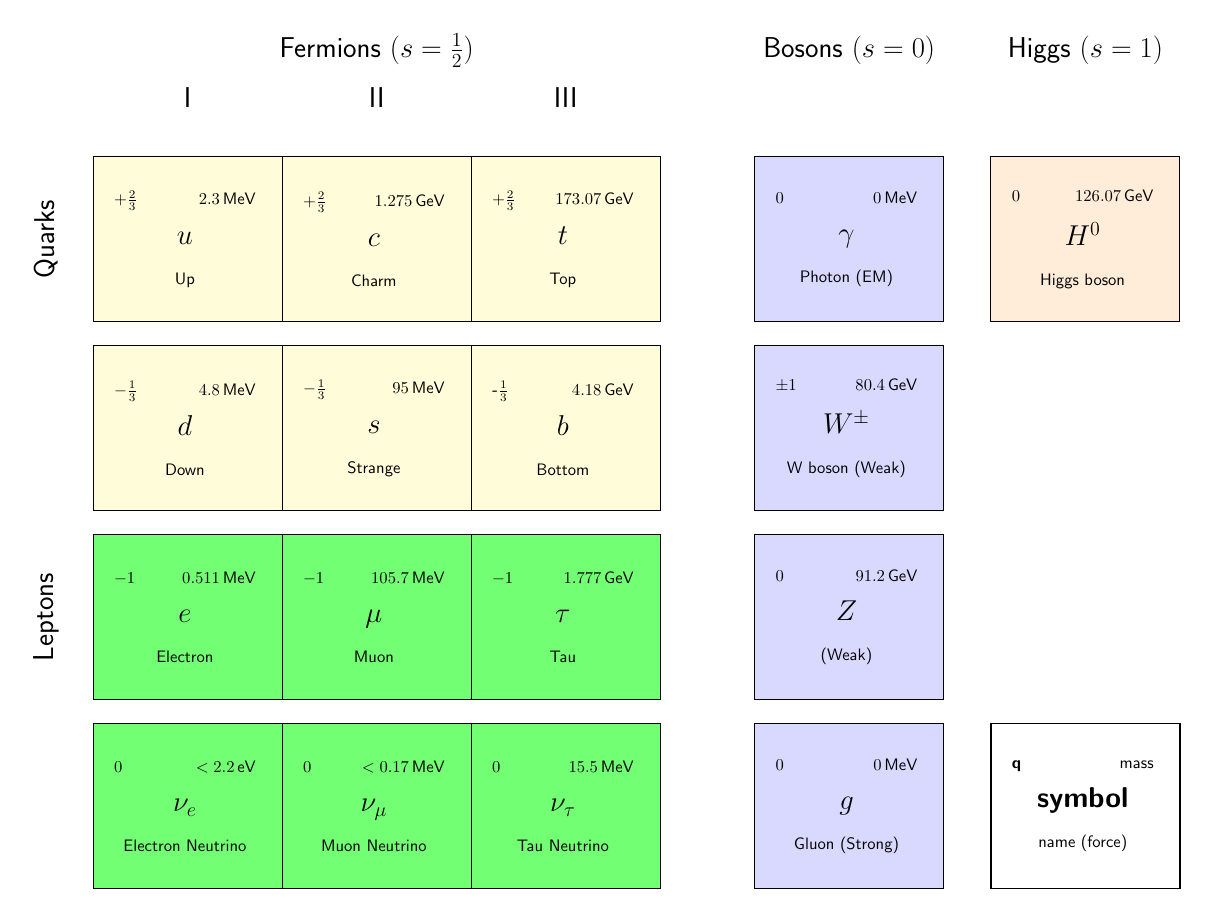
\begin{tikzpicture}[font=\sffamily, scale=0.6, transform shape]
      \tikzstyle{FermionFill} = [fill=yellow!15]
      \tikzstyle{QuarkFill} = [fill=yellow!15]
      \tikzstyle{LeptonFill} = [fill=green!55]
      
      \tikzstyle{Fermion} = [draw=black, FermionFill, minimum width=4cm, minimum height=3.5cm, node distance=4cm]
      
      \tikzstyle{Quark} = [Fermion, QuarkFill]
      \tikzstyle{Lepton} = [Fermion, LeptonFill]

      \tikzstyle{GenerationLabel} = [font={\sffamily\LARGE}, minimum width=2.75cm, node distance=3.0cm]

      \node[name=Up, Quark] {\NaturalElementTextFormat{$+\frac{2}{3}$}{$2.3$\,MeV}{$u$}{Up}};
      \node[name=Down, below of=Up, Quark] {\NaturalElementTextFormat{$-\frac{1}{3}$}{$4.8$\,MeV}{$d$}{Down}};
      \node[name=Charm, right of=Up, Quark] {\NaturalElementTextFormat{$+\frac{2}{3}$}{$1.275$\,GeV}{$c$}{Charm}};
      \node[name=Strange, below of=Charm, Quark] {\NaturalElementTextFormat{$-\frac{1}{3}$}{$95$\,MeV}{$s$}{Strange}};
      \node[name=Top, right of=Charm, Quark] {\NaturalElementTextFormat{$+\frac{2}{3}$}{$173.07$\,GeV}{$t$}{Top}};
      \node[name=Bottom, below of=Top, Quark] {\NaturalElementTextFormat{-$\frac{1}{3}$}{$4.18$\,GeV}{$b$}{Bottom}};
      
      \node[name=Electron, below of=Down, Lepton] {\NaturalElementTextFormat{$-1$}{$0.511$\,MeV}{$e$}{Electron}};
      \node[name=Electron Neutrino, below of=Electron, Lepton] {\NaturalElementTextFormat{$0$}{$<2.2$\,eV}{$\nu_{e}$}{Electron Neutrino}};
      \node[name=Muon, right of=Electron, Lepton] {\NaturalElementTextFormat{$-1$}{$105.7$\,MeV}{$\mu$}{Muon}};
      \node[name=Muon Neutrino, below of=Muon, Lepton] {\NaturalElementTextFormat{$0$}{$<0.17$\,MeV}{$\nu_{\mu}$}{Muon Neutrino}};
      \node[name=Tau, right of=Muon, Lepton] {\NaturalElementTextFormat{$-1$}{$1.777$\,GeV}{$\tau$}{Tau}};
      \node[name=Tau Neutrino, below of=Tau, Lepton] {\NaturalElementTextFormat{$0$}{$15.5$\,MeV}{$\nu_{\tau}$}{Tau Neutrino}};

      \node[name=Generation1, above of=Up, GenerationLabel] {I};
      \node[name=Generation2, above of=Charm, GenerationLabel] {II};
      \node[name=Generation3, above of=Top, GenerationLabel] {III};

      \node[name=FermionName, above of=Generation2, GenerationLabel, node distance=1cm] {Fermions $(s=\frac{1}{2})$};
  
      \node[name=LeptonLabel, left of=Electron, GenerationLabel, rotate=90]{Leptons};
      \node[name=QuarkLabel, left of=Up, GenerationLabel, rotate=90]{Quarks};

      \tikzstyle{BosonFill} = [fill=blue!15]
      \tikzstyle{HiggsFill} = [fill=orange!15]
      \tikzstyle{Boson} = [draw=black, BosonFill, minimum width=4cm, minimum height=3.5cm, node distance=4cm]
      \tikzstyle{Higgs} = [Boson, HiggsFill]

      \node[name=Photon, Boson, right of=Top, xshift=2cm] {\NaturalElementTextFormat{$0$}{$0$\,MeV}{$\gamma$}{Photon (EM)}};
      \node[name=W, below of=Photon, Boson] {\NaturalElementTextFormat{$\pm1$}{$80.4$\,GeV}{$W^{\pm}$}{W boson (Weak)}};
      \node[name=Z, below of=W, Boson] {\NaturalElementTextFormat{$0$}{$91.2$\,GeV}{$Z$}{\ZbosonText{} (Weak)}};
      \node[name=Gluon, below of=Z, Boson] {\NaturalElementTextFormat{$0$}{$0$\,MeV}{$g$}{Gluon (Strong)}};
      \node[name=Higgs, right of=Photon, Higgs, xshift=1cm] {\NaturalElementTextFormat{$0$}{$126.07$\,GeV}{$H^{0}$}{Higgs boson}};
      \node[name=Legend, right of=Gluon, Boson, fill=white, xshift=1cm] {\NaturalElementTextFormat{q}{mass}{symbol}{name (force)}};
      
      \node[name=QuarkLabel, above of=Photon, GenerationLabel, node distance=4cm]{Bosons $(s=0)$};
      \node[name=QuarkLabel, above of=Higgs, GenerationLabel, node distance=4cm]{Higgs $(s=1)$};
    \end{tikzpicture}
    \caption{A summary of all elementary particles described by the SM\cite{Theory:PDGBooklet}. Note the various groupings and divisions including by spin, generation and particle type. Within the fermion sector the quarks are shown in yellow and the leptons are shown in green. These are grouped into three different generations traditionally denoted by roman numerals. The force mediators known as gauge bosons are shown in blue and finally the recently discovered Higgs boson with a spin of zero.} \label{tab:TheorySmParticles}
\end{table}

%% Table of Forces
\begin{table}[htbp]
  \centering  
    \begin{tabular}{|c|c|c|}
    \hline
    Name & Relative Strength & Boson \\ \hline \hline
    Strong & $10^{38}$ & Gluons \\
    Electronmagnetic & $10^{36}$ & Photon \\ 
    Weak & $10^{25}$ & \Wboson and \Zboson \\
    Gravity & $1$ & Graviton* \\ \hline
    \end{tabular}
    \caption{A summary of the four fundamental forces ordered by relative strength. These are approximate relative strengths for the purpose of demonstrating the hierarchy of forces as a function of their strength. A more accurate determination of the interaction strength depends on the details of the interaction itself. Note however the order-of-magnitude differences in the relative strengths of these forces. Note that the graviton is the theoretical boson responsible for mediating gravitational interactions, it is not part of the SM.} \label{tab:TheoryForces} 
\end{table}

\section{Quantum Electrodynamics}

The interaction of particles via the electromagnetic force is described by Quantum Electrodynamics or QED. These interactions are mediated by the massless neutral boson known as the photon and the strenght of the interaction is characterized by the fine-structure constant $\alpha$. All electrically charged fermions are allowed to interact, since the photon itself is not charged, no self-interaction is allowed within QED. Figure~\ref{fig:TheorySimpleQED} shows the single vertex described by QED, where two fermions interact via a photon. Note that the electric charge is conserved across the vertex, so for example $\gamma\rightarrow e^{+}e^{+}$ is not allowed within QED.

%% Simple QED Vertex
\begin{figure}
  \centering
  \begin{fmffile}{simpleqed}
    \begin{fmfgraph*}(100,80)

    \fmftop{fi,fo} \fmfbottom{Photon}
    \fmf{fermion}{fi,vx1,fo}
    \fmf{boson,label=$\gamma$}{vx1,Photon}
    \fmflabel{$f$}{fi} \fmflabel{$f$}{fo}
    \fmfdot{vx1}

  \end{fmfgraph*}
  \end{fmffile}
  \caption{The interaction vertex described by QED. One can obtain all possible vertex shapes by rotating this basic vertex and assigning the appropriate electric charge and making sure to conserve lepton number across the vertex.} \label{fig:TheorySimpleQED}
\end{figure}

By combining different forms of this vertex one can build every possible QED interaction. For example an $e^{+}e^{-}$ pair can annihilate to create energy in the form of a photon as shown in Fig.~\ref{fig:TheoryQEDTreeA} and then subsequently decay into an additional $e^{+}e^{-}$ pair. Electrons can scatter by emitting a photon which is then absorbed by a positron as shown in Fig.~\ref{fig:TheoryQEDTreeB} this process is known as Bhabha scattering.

%% Example Tree Level Diagrams
\begin{figure}
  \begin{minipage}[b]{.48\textwidth}
    \centering
    \begin{fmffile}{TheoryQEDTreeA}
    \fmfframe(5,17)(20,17) {
    \begin{fmfgraph*}(100,80)
      \fmfleft{ele1,pos1}
      \fmfright{ele2,pos2}
      \fmf{fermion}{ele1,v1}
      \fmf{fermion}{v1,pos1}
      \fmf{photon,label=$\gamma$}{v1,v2}
      \fmf{fermion}{ele2,v2}
      \fmf{fermion}{v2,pos2}
      \fmflabel{$e^{+}$}{pos1} \fmflabel{$e^{+}$}{pos2}
      \fmflabel{$e^{-}$}{ele1} \fmflabel{$e^{-}$}{ele2}
      \fmfdot{v1,v2}
    \end{fmfgraph*}
    }
    \end{fmffile}
    \subcaption{Electron-Positron pair annihilation mediated by a photon.} \label{fig:TheoryQEDTreeA}
  \end{minipage}
  \,
  \begin{minipage}[b]{.48\textwidth}
    \centering
    \begin{fmffile}{TheoryQEDTreeB}
    \fmfframe(5,17)(20,17) {
      \begin{fmfgraph*}(100,80)
        \fmfleft{ele1,pos1}
        \fmfright{ele2,pos2}
        \fmf{fermion}{ele1,v1}
        \fmf{fermion}{v1,ele2}
        \fmf{photon,label=$\gamma$}{v1,v2}
        \fmf{fermion}{v2,pos1}
        \fmf{fermion}{pos2,v2}
        \fmflabel{$e^{+}$}{pos1} \fmflabel{$e^{+}$}{pos2}
        \fmflabel{$e^{-}$}{ele1} \fmflabel{$e^{-}$}{ele2}
      \end{fmfgraph*}
    }
    \end{fmffile}
    \subcaption{Electron-Positron pair scattering via the emission of a photon.} \label{fig:TheoryQEDTreeB}
  \end{minipage}
  \caption{Feynman diagrams of the process $e^{+}e^{-}\rightarrow e^{+}e^{-}$ allowed in QED. Note that these are the simplest diagrams, also known as tree level diagrams, and additional vertices can be added to produce higher-order diagrams of the same process.}
  \label{fig:TheoryQEDTree}
\end{figure}

\section{Quantum Chromodynamics}

Interactions via the strong force are described in the theory of Quantum Chromodynamics or QCD. These interactions are mediated by a set of massless neutral bosons known as gluons. QCD introduces the concept of colour, which similarly to electrical charge, determines the possible interactions that can occur via the strong force. Colour can take three states: red (antired), blue (antiblue), green (antigreen). For example both quarks and gluons possess colour and as a result gluons, unlike photons, can self-interact (Figure~\ref{fig:TheoryQCDVertexes})). As with electrical charge, colour-charge must also be conserved. Thus in the scattering process $q\rightarrow q+g$ shown in Figure~\ref{fig:TheoryQCDColour} the flavour of the quark may not change but the colour-charge does and the gluon carries away the difference in colour. There are eight different gluons that can participate in QCD interactions each with a different colour-charge combination. \comment{EXPLAIN WHAT YOU MEAN BY THIS}Note that there is a ninth combination ($R\overline{R} + G\overline{G}+B\overline{B}$) which is overall colorless so it cannot take part in interactions.

In an analogous fashion to screening which occurs with electric charges, quark-antiquark pairs act like dipoles which screen the true colour charge of the central quark. However since gluons also carry colour, they cause the opposite effect (anti-screening) to amplify and change the observed colour of the quark. Which effect wins out depends on the number of colours in the theory and the number of quark flavours. As it is with three colour states and six different quark flavours, anti-screening is the overall dominant effect. As a result the colour potential decreases with distance and quarks experience very little potential when very near to each other. This effect is known as asymptotic freedom and results in quarks only existing within colorless bound states known as hadrons.

Hadrons can be divided into two categories: mesons, which contain a quark and an antiquark ($q\overline{q}$); and baryons which are made of three quarks (or antiquarks) each with a different (anti)colour-charge to result in a colourless composite particle. Common examples of baryons are protons (uud) and neutrons (udd) which are the building blocks of atomic nuclei. While $\pi^{0} (u\overline{u}/d\overline{d})$ is a commonly produced meson in hadron colliders. Note that due to the quark configuration, baryons have baryon number B=+1 while mesons have B=0.
  
%% Self-interacting QCD Gluon vertices
\begin{figure}
  \begin{minipage}[b]{.32\textwidth}
    \begin{fmffile}{ColourQCD}
    \begin{fmfgraph*}(100,80)
    \fmftop{qin,qout} \fmfbottom{glu}
    \fmf{quark}{qin,vertex1,qout}
    \fmf{gluon,label=$g$}{vertex1,glu}
    \fmfdot{vertex1}
    \fmflabel{$q$}{qin} \fmflabel{$q$}{qout}
    \end{fmfgraph*}
    \end{fmffile}
    \subcaption{Quark-gluon vertex.} \label{fig:TheoryQCDColour}
  \end{minipage}
  \,
  \begin{minipage}[b]{.32\textwidth}
    \centering
    \begin{fmffile}{selfqcd4}
    \begin{fmfgraph*}(100,80)
      \fmfleft{glu1,glu2}
      \fmfright{glu3,glu4}
      \fmf{gluon}{glu1,vertex1} \fmf{gluon}{glu2,vertex1}
      \fmf{gluon}{vertex1,glu3} \fmf{gluon}{vertex1,glu4}
      \fmfdot{vertex1}
    \end{fmfgraph*}
    \end{fmffile}
    \subcaption{Four-gluon vertex} \label{fig:TheoryQCDFourGluon}
  \end{minipage}
  \,
  \begin{minipage}[b]{.32\textwidth}
    \centering
    \begin{fmffile}{selfqcd3}%
    \begin{fmfgraph*}(100,80)
      \fmfleft{glu1}
      \fmfright{glu3,glu4}
      \fmf{gluon}{glu1,vertex1}
      \fmf{gluon}{vertex1,glu3} \fmf{gluon}{vertex1,glu4}
      \fmfdot{vertex1}
    \end{fmfgraph*}
    \end{fmffile}
    \subcaption{Three-gluon vertex} \label{fig:TheoryQCDThreeGluon}
  \end{minipage}
  \caption{Diagrams of the fundamental interaction vertices described by quantum chromodynamics.} \label{fig:TheoryQCDVertexes}
\end{figure}

\section{Weak Interactions}

The final type of interaction involves the so-called weak force. The weak force is responsible for $\beta^{-}$ decay ($n\rightarrow p +e^{-}+\overline{\nu}_{e}$) and $\beta^{+}$ decay. Interactions via the Weak force are mediated by a single neutral massive boson and two charged massive bosons. Since the bosons responsible for weak interactions are massive, the range of interaction is very short, unlike electromagnetic interactions via a massless photon.

All fermions can take part in interactions via the Weak force. Let us consider weak interactions involving only leptons. The Weak neutral vertex is very similar to the basic vertex seen in QED (\ref{fig:TheorySimpleQED}) A valid interactions via the weak force is then formed by combining these simple vertices (Figure~\ref{fig:TheoryWeakVertexes}) while taking care to conserve electric charge and lepton flavour. An example of a leptonic weak interaction is muon decay ($\mu\rightarrow \nu_{\mu}W^{-}\rightarrow \nu_{\mu}e^{-}\overline{\nu}_{e}$) shown in Figure~\ref{fig:TheoryMuonDecay}.

%% Weak Neutral Vertexes
\begin{figure}
  \begin{minipage}[b]{.32\textwidth}
    \centering
    \begin{fmffile}{WeakNeutral}
    \begin{fmfgraph*}(100,80)
      \fmftop{fi,fo} \fmfbottom{ZBoson}
      \fmf{fermion}{fi,vx1,fo}
      \fmf{boson,label=$Z^{0}$}{vx1,ZBoson}
      \fmflabel{$f$}{fi} \fmflabel{$\overline{f}$}{fo}
      \fmfdot{vx1}
    \end{fmfgraph*}
    \end{fmffile}
    \subcaption{Neutral current weak vertex} \label{fig:TheoryWeakNeutralFermions}
  \end{minipage}
  \,
  \begin{minipage}[b]{.32\textwidth}
    \centering
    \begin{fmffile}{WeakCharged}
    \begin{fmfgraph*}(100,80)
      \fmftop{fi,fo} \fmfbottom{WBoson}
      \fmf{fermion}{fi,vx1,fo}
      \fmf{boson,label=$W$}{vx1,WBoson}
      \fmflabel{$\ell$}{fi} \fmflabel{$\nu_{\ell}$}{fo}
      \fmfdot{vx1}
    \end{fmfgraph*}
    \end{fmffile}
    \subcaption{Charged current vertex involving leptons} \label{fig:TheoryWeakChargedLeptons}
  \end{minipage}
  \,
  \begin{minipage}[b]{.32\textwidth}
    \centering
    \begin{fmffile}{WeakChargedQuark}
    \begin{fmfgraph*}(100,80)
      \fmftop{fi,fo} \fmfbottom{WBoson}
      \fmf{fermion}{fi,vx1,fo}
      \fmf{boson,label=$W$}{vx1,WBoson}
      \fmflabel{$\overline{q}$}{fi} \fmflabel{$q'$}{fo}
      \fmfdot{vx1}
    \end{fmfgraph*}
    \end{fmffile}
    \subcaption{Charged current vertex involving quarks} \label{fig:TheoryWeakChargedQuarks}
  \end{minipage}

  \caption{The neutral current and charged current vertices allowed via the Weak force. Where $f$ can be an $e$, $\mu$ or $\tau$ and $\nu_{\ell}$ is the corresponding lepton neutrino of the same flavour. 
  One can obtain all possible interaction vertices by rotating these basic vertices and assigning the appropriate electric charge and making sure to conserve lepton flavour across the vertex.}
  \label{fig:TheoryWeakVertexes}
\end{figure}

%% Weak Muon Decay
\begin{figure}
  \centering
  \begin{fmffile}{WeakMuonDecay}
    \begin{fmfgraph*}(90,80)
      \fmfleft{muon}
      \fmfright{numu,e,nue}
      \fmf{fermion}{muon,vx1,numu}
      \fmf{boson}{vx1,vx2}
      \fmf{fermion}{nue,vx2,e}
      \fmfdot{vx1,vx2}
    \end{fmfgraph*}
  \end{fmffile}
  \caption{Neutral current weak scattering vertex} \label{fig:TheoryMuonDecay}
\end{figure}

Let us consider weak interactions involving quarks. The neutral vertex is similar to that of the leptonic version, a quark can emit a \ZbosonText{} or a \ZbosonText{} can decay forming a quark-antiquark pair. The charged current then changes the flavour of an up-type quark into a down-type quark (or vice-versa) with a \WbosonText{} of the appropriate charge (Figure~\ref{fig:TheoryWeakChargedQuarks}). It is possible for a Weak interaction to change the flavour of a quark across families. A well known example of such an interaction is Kaon decay ($K^{+}\rightarrow \mu^{+}\nu_{\mu}$). In order to account for this interaction and preserve the universality of weak interactions, Nicola Cabibbo postulated that the states that the states that couple to the charged current are really a mixture of 'rotated' quark states:

\begin{equation}
\begin{pmatrix}
  u \\
  d' \\
\end{pmatrix}
\begin{pmatrix}
  c \\
  s' \\
\end{pmatrix}
\begin{pmatrix}
  t \\
  b' \\
\end{pmatrix}
\end{equation}

where

\begin{subequations}
  \begin{equation}
  \label{eq:TheoryWeakQuarkMixingEq1}
  d'=d\cos\theta_{c} + s\sin\theta_{c}
  \end{equation}
  \begin{equation}
  \label{eq:TheoryWeakQuarkMixingEq2}
  s'=-d\sin\theta_{c} + s\cos\theta_{c}
  \end{equation}
\end{subequations}

This introduces an arbitrary parameter into the theory known as the quark mixing angle or the Cabibbo angle, named after Nicola Cabibbo who developed the phenomenon of quark mixing. The introduction of quark mixing has the effect of attenuating the interaction strength at vertices involving multiple quark generations. Interactions which cross one generation ($u\rightarrow s$) are said to be Cabibbo Suppressed while those that cross two generations ($u\rightarrow b$) are Doubly Cabibbo suppressed.

Taking into account the three quark generations, quark mixing can be expressed in matrix notation as shown in Equation~\ref{eq:TheoryWeakQuarkMixingMatrix}. This unitary matrix is known as the Cabibbo-Kobayashi-Maskawa Matrix (CKM Matrix) after Cabibbo which initially postulated quark mixing and Makoto Kobayashi and Toshihide Maskawa who later added an additional generation, containing the top and bottom quarks, to the matrix.

\begin{equation}
\label{eq:TheoryWeakQuarkMixingMatrix}
\begin{pmatrix}
  d' \\
  s' \\
  b' \\
\end{pmatrix}
=
V_{CKM}
\begin{pmatrix}
  d \\
  s \\
  b \\
\end{pmatrix}
=
\begin{pmatrix}
  V_{ud} & V_{us} & V_{ub} \\
  V_{cd} & V_{cs} & V_{cb} \\
  V_{td} & V_{ts} & V_{tb} \\
\end{pmatrix}
\begin{pmatrix}
  d \\
  s \\
  b \\
\end{pmatrix}
\end{equation}

The elements of the CKM matrix have been measured and the latest accepted results are summarized in \ref{eq:TheoryWeakCKM}. The interaction strength is then proportional to $|V_{ij}|^{2}$. Including all three generations the sum of all possible transitions from a given quark, q, is unity:

\begin{equation} 
\label{eq:TheoryWeakMixingTotal}
\sum|V_{qi}|^{2}=1
\end{equation}

Note that the term $V_{tb}$ is approximately unity and by far dominates over the other $V_{tj}$ terms. This means that the top-quark transitions almost exclusively into a \bquark{} ($t\rightarrow Wb$) with transitions $t\rightarrow Ws$ and $t\rightarrow Wd$ being exceedingly rare. The Soft Muon Tagger which is the focus of this thesis relies on Weak semileptonic decays of \bquark{}s. From \ref{eq:TheoryWeakCKM} one can see that the transition $b\rightarrow c$ dominates over $b\rightarrow u$.

\begin{equation}
\label{eq:TheoryWeakCKM}
V_{CKM}
=
\begin{pmatrix}
  0.97427\pm0.00015 & 0.22534\pm0.00065 & 0.00351\substack{+0.00015\\-0.00014} \\
  0.22520\pm0.00065 & 0.97344\pm0.00016 & 0.0412\substack{+0.0011\\-0.0005} \\
  0.00867\substack{+0.00029\\-0.00031} & 0.0404\substack{+0.0011\\-0.0005} & 0.999146\substack{+0.000021\\-0.000046} \\
\end{pmatrix}
\end{equation}

An additional unique feature of Weak interactions is that the charge conjugation-parity (CP) symmetry is violated. The operator C denotes the change of a particle by its antiparticle partner and P denotes a reversal of helicity (the projection of spin onto the momentum of a particle). A clear violation of C and P was observed in the radioactive decay of Cobalt-60, where the resulting electrons were preferentially emitted in the opposite direction of the nuclear spin of the Cobalt. Thus weak currents only couple to left-handed neutrinos (or right-handed antineutrinos) this is then a violation of parity. Additionally charge symmetry is also violated since a left-handed neutrino is preferentially picked over a left-handed antineutrino. Finally in 1964 CP violation was observed in the decay of neutral kaon.

Thus the probability of $\overline{a}\rightarrow \overline{b}$ is not equal to that of $a\rightarrow b$. The existence of CP violation has interesting consequences for the formation of the early universe. The preferential production of matter over antimattter in CP violating interactions would shift the balance in favour of matter resulting in a universe similar to our own.

\subsection{Electroweak Unification and the Higgs mechanism}


